\documentclass[10pt,a4paper]{article}
\usepackage[margin=2.2cm]{geometry}
\usepackage[T1]{fontenc}
\usepackage{lmodern}
\usepackage{microtype}
\usepackage{amsmath}
\usepackage{booktabs}
\usepackage{longtable}
\usepackage{tabularx}
\usepackage{array}
\usepackage{graphicx}
\usepackage{xcolor}
\usepackage{caption}
\usepackage{enumitem}
\usepackage[hidelinks]{hyperref}
\captionsetup{font=small,labelfont=bf}
\setlist{nosep,leftmargin=1.4em}
\newcolumntype{L}{>{\raggedright\arraybackslash}X}
\definecolor{ok}{HTML}{0ca30c}\definecolor{bad}{HTML}{d03b3b}\definecolor{part}{HTML}{c98500}
\newcommand{\OK}{\textcolor{ok}{\textbf{Conforms}}}
\newcommand{\NO}{\textcolor{bad}{\textbf{Does not conform}}}
\newcommand{\PART}{\textcolor{part}{\textbf{Partial}}}
\newcommand{\NT}{\textbf{Not tested}}
\newcommand{\code}[1]{\texttt{\small #1}}

\title{\textbf{How far does Pinocchio-EP follow ANSI/ASHRAE Standard 140-2023?}\\[3pt]
\large A method-of-test assessment against the 2023 standard, Addendum~a (time-series acceptance criteria)\\
and Addendum~b (ETNA empirical validation), with measured results}
\author{ERGO Energy LLP --- Pinocchio-EP engineering\\\small Assessment date: 26 October 2026}
\date{}

\begin{document}
\maketitle

\begin{abstract}
\noindent
Pinocchio-EP is a web building-energy modelling application that writes EnergyPlus input files from a
document-driven wizard and runs an unmodified EnergyPlus~26.1 engine. ANSI/ASHRAE Standard~140-2023 defines the
method of test for building performance simulation \emph{software}, which it explicitly defines as the calculation
engine \emph{together with} its user interface; results from one interface cannot be used as a proxy for another
interface on the same engine. We therefore tested Pinocchio-EP itself. We (i) reduced the 2023 standard and its two
addenda to a requirements checklist, (ii) audited Pinocchio-EP's code against every modelling capability the test
cases require, (iii) generated the complete Section~7 thermal-fabric suite (21 conditioned cases plus free-float
cases) \emph{through Pinocchio-EP's own IDF emitter} at three input levels and scored it against the Annex~A3
acceptance criteria as revised by Addendum~a (single-value ranges plus hourly Pearson/RMSE criteria), and
(iv) ran the six Addendum~b ETNA empirical cases on Pinocchio-EP's engine, both directly and through Pinocchio-EP's
IDF import path.
With faithful inputs (supplied through IDF import or programmatic passthrough), Pinocchio-EP places
\textbf{34/34} low-mass and \textbf{28/28} high-mass range cases inside the acceptance ranges (30 and 25 required).
With only the inputs its graphical interface can create, the low-mass group still passes (33/34) but the
\textbf{high-mass group fails (21/28)}, chiefly because the interface represents every window by a U-factor/SHGC
``simple glazing'' object. A dead GUI field that leaves the wind terrain hard-coded to ``City'' alone pushes Case~900
(faithful inputs) and Case~600 (GUI inputs) out of range. On the ETNA tests the engine reproduces measured heater
power within the measurement uncertainty (+0.06\,\%, +0.50\,\%, $-$0.04\,\%, $-$0.04\,\%), but Pinocchio-EP's import
path silently caps the time step at 4 per hour and inflates the predicted heater power by a factor of 4 to 11.
Sections~6, 8, 9, 10, 11 and 12 were not exercised, no Standard~140 output reports exist, and Pinocchio-EP therefore
cannot today claim conformance. We list every non-conformance with code evidence and the fix for each.
\end{abstract}

\section{Introduction}
Standard~140 is the consensus method of test used by energy codes and rating programs (for example the performance paths of ASHRAE~90.1) to qualify simulation
programs. Its 2023 edition contains Class~I analytical, comparative and empirical tests for weather processing
(Section~6), building thermal fabric (Section~7), ground coupling (Section~8), cooling equipment (Section~9),
heating equipment (Section~10) and air-side HVAC (Section~11), plus Class~II tests for simplified tools
(Section~12). Addendum~a (approved 29 August 2025) adds hourly time-series acceptance criteria to the
thermal-fabric groups and raises the minimum pass counts. Addendum~b (approved 24 April 2026) adds Section~13, the
standard's first empirical validation tests, based on measured heater power in the twin ETNA test cells
(EDF, France).

Pinocchio-EP does not implement its own heat-balance solver; every simulation is performed by EnergyPlus~26.1.0
(build \code{6f2e40d102}). It would be tempting to cite EnergyPlus's published Standard~140 results. The standard
forbids this. Its Section~3.1 defines \emph{software} as ``a package consisting of the user interface, input
interface, calculation engine, and output interface'', and normative Annex~A3 states that ``the testing of software
only meets the requirements of this annex for that software and cannot be used as a proxy for documenting compliance
of another software that uses the same calculation engine but a different user interface''. Addendum~a repeats
this rule unchanged. What matters is therefore whether Pinocchio-EP's interface and IDF writer let a modeller
express the specified inputs, preserve them on the way to the engine, and report the specified outputs.

This paper answers that question with measurements rather than by inspection alone. Section~\ref{sec:std}
summarises the requirements, Section~\ref{sec:pin} the relevant architecture, Section~\ref{sec:method} the test
method, Section~\ref{sec:res} the results, Section~\ref{sec:matrix} a clause-by-clause conformance matrix, and
Section~\ref{sec:gaps} every point where Pinocchio-EP does \emph{not} follow the standard, with the remedy.

\section{What Standard 140-2023 and its addenda require}\label{sec:std}
\subsection{General procedure (Section 5 and Annex A2)}
\begin{itemize}
\item \textbf{Modelling rules (5.1.1).} Local standard time, with hour~1 = 00:00--01:00 and no daylight saving or
holidays; consistent modelling methods and \emph{consistent numerical settings} across a test suite; equivalent
inputs only with a mathematical, physical or logical basis; nonspecified inputs only in four listed topics
(constant surface coefficients, interior solar fractions, air density at altitude); full annual runs for Sections~6
and 7; arbitrary tuning of inputs or code to match results is prohibited. Addendum~b adds 5.1.1.9: time steps and
tolerances follow the software implementation, with a warning that thin or light layers can be inaccurate or
unstable at large time steps.
\item \textbf{Reporting (5.1.2, Annex A2).} Results must be entered in the normative \code{Std140\_*\_Output}
workbooks, accompanied by an \code{S140outNotes} report with blocks A (software name and a unique version
identifier), B (alternative methods), C (equivalent methods), D (nonspecified inputs), E (omitted cases),
F (unreleased source changes) and G (anomalous results). Input files and processed weather data must be archived.
\end{itemize}

\subsection{Acceptance criteria (Annex A3 as revised by Addendum a)}
Acceptance ranges exist only for Class~I test groups: thermal fabric low mass, thermal fabric high mass, cooling
equipment (CE300--CE440), heating equipment (HE210--HE230) and air-side equipment (AE200--AE400). Within each group
the software passes when enough results fall inside the ranges (Table~\ref{tab:passcounts}). Addendum~a adds, for each
thermal-fabric case listed in Tables~A3-3 and A3-6, the 24~hourly loads on 1~February and 14~July. These are
compared with a representative curve (the hourly median of the reference programs). A day passes when the Pearson
correlation exceeds 0.879 \emph{and} the RMSE is below a case-specific limit. Sections~6, 8, 12 and 13 have no
acceptance ranges; their comparisons are informative.

\begin{table}[h]\centering\small
\caption{Annex A3 pass criteria after Addendum a (Table A3-10).}\label{tab:passcounts}
\begin{tabular}{lccc}\toprule
Test group & Range tables & Range cases & Minimum in range\\\midrule
Thermal fabric, low mass & A3-1, A3-3 & 34 (21 + 13 day-curves) & 30\\
Thermal fabric, high mass & A3-4, A3-6 & 28 (19 + 9 day-curves) & 25\\
Cooling equipment & A3-7 & 14 & 12\\
Heating equipment & A3-8 & 6 & 5\\
Air-side equipment & A3-9 & 54 & 48\\\bottomrule
\end{tabular}
\end{table}

\subsection{Section 13 (Addendum b): ETNA empirical validation}
Six cases (ET110A1, ET110B1, ET100A1, ET100B1, ET100A3, ET100B3) model a fully guarded test cell: measured
guard-zone air temperatures are imposed on every surface, the cell is held at the hourly measured set point
(about 35\,\textdegree C), the measured fan energy is a convective gain, and the model's heater energy $Q_{htr}$ is
compared with the measured value over a ``best steady-state'' window (18~h for ET110, 55~h for ET100). The ``1''
cases prescribe constant combined surface coefficients; the ``3'' cases require the modeller's automatic interior
convection and radiation algorithms. The measured 2-sigma uncertainty $u(Q_{htr})$ is 0.7--1.0\,\%. The comparison
is informative: no pass/fail range is defined.

\section{Pinocchio-EP architecture relevant to Standard 140}\label{sec:pin}
A project is an ordered array of typed IDF objects plus authored geometry, loads and HVAC. \code{exportIdf()}
(\code{src/product/idfProject.js}) assembles the runnable IDF and the browser posts it to \code{POST /api/run}. The
server writes the text verbatim to \code{in.idf} and runs \code{energyplus -x [-r] -w <epw>}. There is no
server-side rewriting, and the engine is the official NREL build, verified by version check in the Dockerfile.
A user can supply inputs by three routes, and the distinction drives most findings:
\begin{enumerate}
\item \textbf{GUI authoring.} Wizard steps, a construction builder from a material library, a loads editor, HVAC
templates, and an ``All model objects'' editor that can \emph{edit fields of existing objects but cannot create
objects}.
\item \textbf{IDF import.} The parsed file becomes the source of truth and is re-serialised with a small set of
rewrites. Among them, the time step is capped at 4 per hour (\code{src/product/idfSync.js:168-171}).
\item \textbf{Programmatic passthrough.} Objects added to \code{project.model} are emitted verbatim. This route is
available to the agent layer and scripts, not to GUI users.
\end{enumerate}

\section{Method}\label{sec:method}
\subsection{Requirements and code audit}
The standard and both addenda were reduced to a cited requirements digest (every clause with its source line). In
parallel, the Pinocchio-EP front end, back end and engine wrapper were audited read-only against a capability
checklist for each test section, recording file and line evidence. Each capability was classified as supported in
the GUI, supported only through import or passthrough, partial, overridden by a default, or not supported.

\subsection{Section 7 thermal-fabric suite through Pinocchio-EP's emitter}
A Node harness (\code{harness/suite.mjs}) builds every case as a Pinocchio-EP \emph{project} (zones, footprints,
windows, per-face boundary overrides, explicit loads, an ideal-loads HVAC system with per-zone thermostats). It
calls Pinocchio-EP's own \code{exportIdf} and runs the result on the bundled EnergyPlus~26.1 binary, which is
identical to the deployed one. The cases are 600--695, 900--995, 960 (two-zone sunspace with an interzone wall) and
the free-float cases 600FF, 650FF, 680FF, 900FF, 950FF and 980FF. Three input levels were run:
\begin{description}
\item[Faithful (P).] Exact Table~7-2/7-25/7-27/7-29/7-31 materials (solar absorptance 0.6, IR emittance 0.9), layered
glazing from Tables~7-10/7-17/7-21 (\code{WindowMaterial:Glazing} plus air or argon gaps), exact shading geometry
of Figures~7-3/7-5/7-6, a 1700\,m\textsuperscript{3}/h night-ventilation object for 650/950, a 15-minute ramp and
an instantaneous step for 640/940, terrain ``Country'' (open terrain, category~3), full interior and exterior solar
distribution, no DST or holidays. Objects the GUI cannot create were supplied by passthrough.
\item[Import (I).] Each faithful IDF was imported through Pinocchio-EP's \code{importIdf} and re-exported, which is
exactly what happens when a user uploads such a file.
\item[GUI-reachable (G).] Only what a GUI user can produce: the same materials and absorptances (reachable by
building constructions and then editing material fields), terrain and solar distribution set in the objects editor,
but windows as \code{WindowMaterial:SimpleGlazingSystem} with the standard's derived U-factor and SHGC
(2.10/0.769, 1.19/0.440, 5.16/0.864), overhangs and fins limited to Pinocchio-EP's per-window shades, night
ventilation as a scheduled infiltration load, and an hourly setback schedule.
\end{description}
All runs use 4 time steps per hour, Pinocchio-EP's default. Hourly ideal-loads sensible heating and cooling energy
were summed to annual MWh. Peaks were taken as the maximum hourly-integrated value. Feb~1 and Jul~14 hourly net
loads (heating $+$, cooling $-$) were scored against the Addendum~a curves with \code{harness/score.py}.

\paragraph{Weather.} The normative file \code{725650TY.CSV} was not among the materials provided. We used the TMY3
record for the same station, Denver International Airport (WMO 725650, 39.833\,N, 104.650\,W, 1650\,m, UTC$-$7,
identical to Annex Table~A1-1), in EPW form from climate.onebuilding.org. The underlying TMY3 data are the same,
but this file is a substitute. The results are therefore an \emph{indicative pre-test}, not a formal Standard~140
result.

\subsection{Section 13 (ETNA)}
The normative measurement files and weather file of Addendum~b were used. The standard's informative EnergyPlus~23.1
inputs were converted to version~26.1 with the official transition programs, and their \code{Schedule:File}
boundary schedules were rebuilt from the normative CSVs (8784 hourly rows for leap year 2000, preceding-hour
convention, GMT+1). Each case was then run (a) directly on EnergyPlus~26.1 (\code{harness/run\_etna.py}) and
(b) after Pinocchio-EP's import$\rightarrow$export round trip (\code{harness/via\_pinocchio.mjs}). Note that the
README of the accompanying files states that the informative input files ``were used to generate the informative
example results'' and are not to be used for developing new results. Run~(a) is therefore an \emph{engine
diagnosis}, not a Section~13 submission. Run~(b) isolates what Pinocchio-EP's own path does to an otherwise
identical model.

\section{Results}\label{sec:res}
\subsection{Section 7: single-value acceptance ranges}
Table~\ref{tab:single} and Figure~\ref{fig:ranges} give every Annex~A3 single-value range case. The import route
(I) reproduced the faithful route (P) to within 0.000\,MWh in every case. Pinocchio-EP's import path changes
nothing that matters for Section~7 at the default time step, so I is not listed separately.

{\small\setlength{\tabcolsep}{5pt}
\begin{longtable}{llrrrr}
\caption{Annex A3 single-value range cases (annual MWh). $^{\dagger}$ = outside the acceptance range.}\label{tab:single}\\
\toprule Range case & Load & Lower & Upper & Faithful (P = I) & GUI-reachable (G)\\\midrule\endfirsthead
\toprule Range case & Load & Lower & Upper & Faithful (P = I) & GUI-reachable (G)\\\midrule\endhead
600 & Heating & 3.75 & 4.98 & 4.379 & 3.948 \\
600 & Cooling & 5.00 & 6.83 & 5.891 & 6.369 \\
610--600 & Heating & -0.14 & 0.29 & 0.045 & 0.036 \\
610--600 & Cooling & -2.26 & -0.80 & -1.678 & -1.526 \\
620--600 & Heating & -0.08 & 0.40 & 0.176 & 0.151 \\
620--600 & Cooling & -2.24 & -1.64 & -1.951 & -2.117 \\
630--620 & Heating & 0.02 & 0.74 & 0.297 & 0.248 \\
630--620 & Cooling & -1.68 & -0.77 & -1.188 & -1.212 \\
640--600 & Heating & -2.17 & -1.22 & -1.649 & -1.405 \\
640--600 & Cooling & -0.56 & 0.03 & -0.277 & -0.230 \\
650--600 & Cooling & -1.54 & -0.95 & -1.223 & -1.342 \\
660--600 & Heating & -1.07 & -0.16 & -0.624 & -0.278 \\
660--600 & Cooling & -3.09 & -2.50 & -2.772 & -3.065 \\
670--600 & Heating & 0.25 & 2.98 & 1.303 & 1.415 \\
670--600 & Cooling & 0.05 & 0.84 & 0.577 & 0.429 \\
680--600 & Heating & -2.54 & -1.90 & -2.190 & -2.180 \\
680--600 & Cooling & 0.13 & 0.87 & 0.460 & 0.586 \\
685--600 & Heating & 0.33 & 0.77 & 0.578 & 0.592 \\
685--600 & Cooling & 2.70 & 3.31 & 3.092 & 2.998 \\
695--685 & Heating & -2.38 & -1.94 & -2.122 & -2.120 \\
695--685 & Cooling & -0.21 & 0.44 & 0.103 & 0.174 \\
\midrule
900 & Heating & 1.04 & 2.28 & 1.706 & 1.333 \\
900 & Cooling & 2.35 & 2.60 & 2.377 & 2.811$^{\dagger}$ \\
900--910 & Heating & -0.52 & -0.02 & -0.299 & -0.213 \\
900--910 & Cooling & 0.35 & 1.74 & 1.073 & 1.069 \\
920--900 & Heating & 1.51 & 1.92 & 1.724 & 1.623 \\
920--900 & Cooling & 0.08 & 0.48 & 0.262 & 0.109 \\
930--920 & Heating & 0.20 & 1.15 & 0.652 & 0.572 \\
930--920 & Cooling & -1.19 & -0.44 & -0.789 & -0.819 \\
940--900 & Heating & -0.82 & -0.37 & -0.607 & -0.425 \\
940--900 & Cooling & -0.19 & 0.06 & -0.062 & -0.062 \\
950--900 & Cooling & -2.00 & -1.56 & -1.718 & -2.085$^{\dagger}$ \\
960--900 & Heating & 0.96 & 1.12 & 1.083 & 1.153$^{\dagger}$ \\
960--900 & Cooling & -1.81 & -1.27 & -1.528 & -1.819$^{\dagger}$ \\
980--900 & Heating & -1.65 & -1.00 & -1.296 & -1.087 \\
980--900 & Cooling & 1.09 & 1.41 & 1.242 & 1.675$^{\dagger}$ \\
985--900 & Heating & 0.64 & 0.81 & 0.711 & 0.714 \\
985--900 & Cooling & 3.52 & 4.18 & 3.821 & 3.808 \\
995--985 & Heating & -1.83 & -1.07 & -1.398 & -1.298 \\
995--985 & Cooling & 0.63 & 1.15 & 0.899 & 1.089 \\
\bottomrule
\end{longtable}}

\begin{figure}[t]\centering
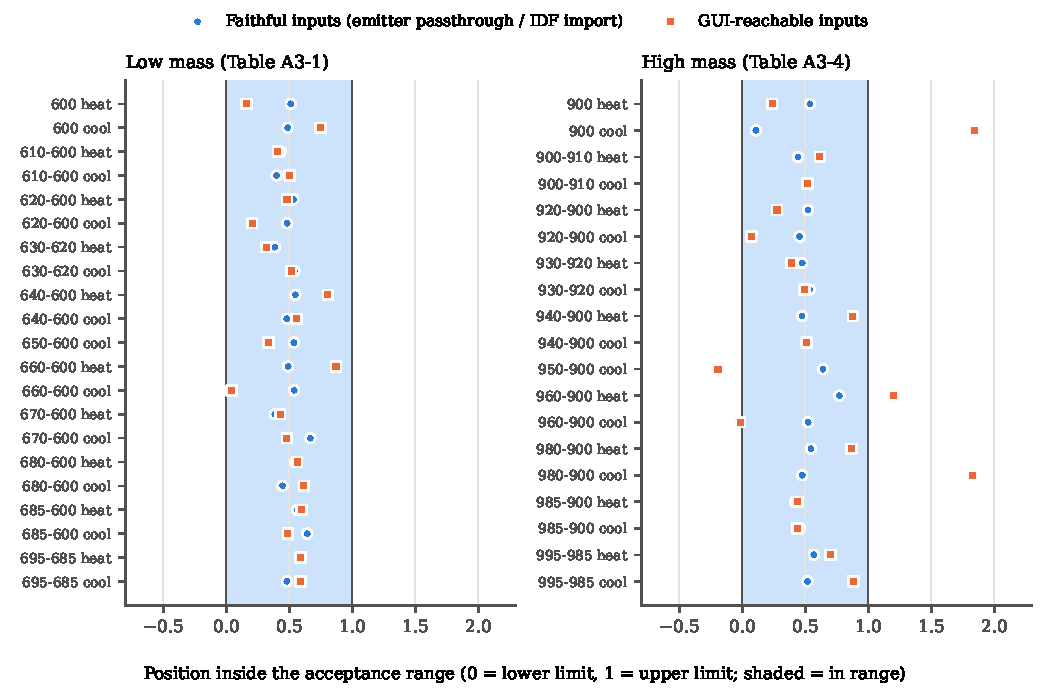
\includegraphics[width=\textwidth]{figures/fig_ranges.pdf}
\caption{Where each result falls inside its acceptance range. The shaded band is the range. With faithful inputs
every result lies well inside it. With GUI-reachable inputs, five high-mass results fall outside.}\label{fig:ranges}
\end{figure}

\subsection{Section 7: Addendum a time-series criteria}
{\small
\begin{longtable}{llrrrrr}
\caption{Hourly-load criteria (Pearson $r > 0.879$ and RMSE $<$ limit, kWh). $^{\dagger}$ = criterion failed.}\label{tab:series}\\
\toprule & & RMSE & \multicolumn{2}{c}{Faithful (P = I)} & \multicolumn{2}{c}{GUI-reachable (G)}\\
Case & Day & limit & $r$ & RMSE & $r$ & RMSE\\\midrule\endfirsthead
\toprule Case & Day & limit & $r$ & RMSE & $r$ & RMSE\\\midrule\endhead
600 & Feb 1 & 0.4194 & 0.999 & 0.111 & 0.999 & 0.295 \\
640 & Feb 1 & 0.6559 & 0.998 & 0.161 & 0.992 & 0.434 \\
660 & Feb 1 & 0.3087 & 0.999 & 0.060 & 0.999 & 0.086 \\
670 & Feb 1 & 0.7881 & 0.999 & 0.141 & 0.999 & 0.272 \\
680 & Feb 1 & 0.3990 & 0.999 & 0.138 & 0.998 & 0.340 \\
685 & Feb 1 & 0.4643 & 0.999 & 0.138 & 0.999 & 0.291 \\
695 & Feb 1 & 0.2069 & 0.999 & 0.168 & 0.999 & 0.332$^{\dagger}$ \\
600 & Jul 14 & 0.1921 & 0.999 & 0.051 & 0.997 & 0.082 \\
660 & Jul 14 & 0.1697 & 0.999 & 0.047 & 0.998 & 0.043 \\
670 & Jul 14 & 0.3018 & 0.998 & 0.078 & 0.998 & 0.087 \\
680 & Jul 14 & 0.2097 & 0.999 & 0.039 & 0.996 & 0.095 \\
685 & Jul 14 & 0.3218 & 0.999 & 0.058 & 0.998 & 0.076 \\
695 & Jul 14 & 0.2001 & 0.999 & 0.051 & 0.998 & 0.069 \\
900 & Feb 1 & 0.3716 & 0.996 & 0.057 & 0.987 & 0.160 \\
940 & Feb 1 & 0.4298 & 0.994 & 0.060 & 0.869 & 0.248$^{\dagger}$ \\
980 & Feb 1 & 0.2969 & 0.985 & 0.095 & 0.980 & 0.306$^{\dagger}$ \\
985 & Feb 1 & 0.4166 & 1.000 & 0.049 & 1.000 & 0.192 \\
995 & Feb 1 & 0.2944 & 0.999 & 0.068 & 0.999 & 0.220 \\
900 & Jul 14 & 0.0967 & 0.998 & 0.046 & 0.996 & 0.062 \\
980 & Jul 14 & 0.0986 & 0.999 & 0.030 & 0.998 & 0.062 \\
985 & Jul 14 & 0.2053 & 0.999 & 0.027 & 0.999 & 0.027 \\
995 & Jul 14 & 0.2468 & 0.999 & 0.029 & 0.999 & 0.029 \\
\bottomrule
\end{longtable}}

\begin{figure}[h]\centering
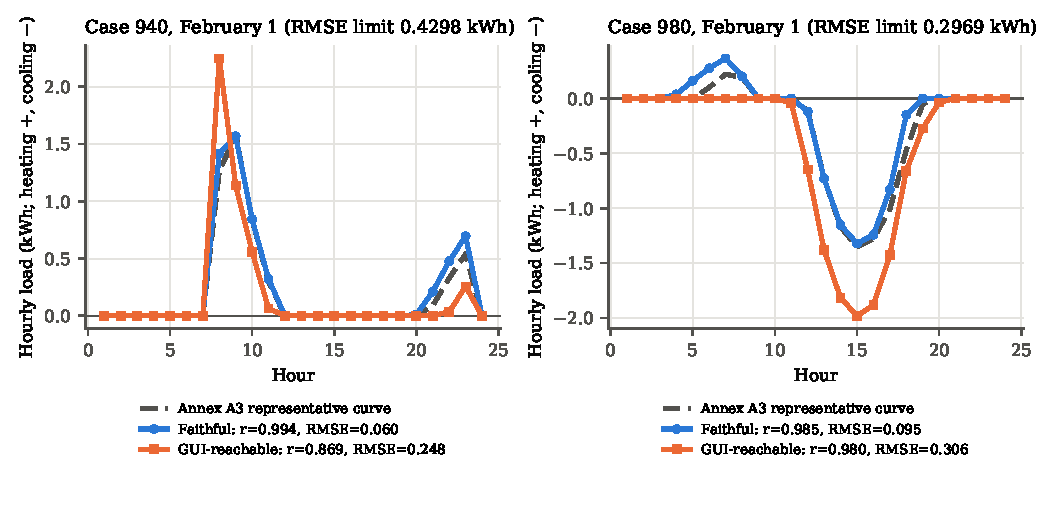
\includegraphics[width=\textwidth]{figures/fig_timeseries.pdf}
\caption{The two high-mass day curves that the GUI-reachable model fails. The simple-glazing representation delays
and lowers the morning recovery load in Case~940 ($r = 0.869$), and over-predicts solar gain and cooling in Case~980
(RMSE 0.306 vs 0.2969).}\label{fig:ts}
\end{figure}

\subsection{Test-group outcome}
\begin{table}[h]\centering\small
\caption{Annex A3 test-group outcome (Section 7 only).}\label{tab:outcome}
\begin{tabular}{lccc}\toprule
Input route & Low mass (need 30/34) & High mass (need 25/28) & Verdict\\\midrule
Faithful, programmatic passthrough (P) & 34/34 & 28/28 & both groups pass\\
Faithful, via IDF import (I) & 34/34 & 28/28 & both groups pass\\
GUI-reachable (G) & 33/34 & \textbf{21/28} & \textbf{high mass fails}\\\bottomrule
\end{tabular}
\end{table}

Table~\ref{tab:annual} lists the base-case annual and peak loads. The free-float temperature extremes
(Table~\ref{tab:ff}) have no acceptance ranges. They are reported for completeness, and to show that free-float
cases can be produced through the emitter, although the GUI refuses to run them (Section~\ref{sec:gaps}).

\begin{table}[h]\centering\small
\caption{Base cases: annual loads (MWh) and hourly-integrated peaks (kW, with time stamp).}\label{tab:annual}
\begin{tabular}{llrrll}\toprule
Case & Route & Heating & Cooling & Peak heating & Peak cooling\\\midrule
600 & Faithful & 4.379 & 5.891 & 3.27 (12/31 24:00) & 6.29 (10/10 13:00) \\
600 & GUI & 3.948 & 6.369 & 3.10 (12/31 24:00) & 6.55 (10/10 13:00) \\
900 & Faithful & 1.706 & 2.377 & 2.74 (02/09 06:00) & 3.05 (10/12 15:00) \\
900 & GUI & 1.333 & 2.811 & 2.56 (02/09 06:00) & 3.31 (10/12 15:00) \\
\bottomrule\end{tabular}
\end{table}

\begin{table}[h]\centering\small
\caption{Free-float zone air temperature (\textdegree C), informative.}\label{tab:ff}
\begin{tabular}{lrrrrrr}\toprule
& \multicolumn{3}{c}{Faithful} & \multicolumn{3}{c}{GUI-reachable}\\
Case & max & min & mean & max & min & mean\\\midrule
600FF & 62.4 & -13.0 & 24.7 & 66.3 & -12.6 & 26.4 \\
650FF & 60.9 & -17.1 & 18.3 & 63.9 & -17.0 & 18.8 \\
680FF & 70.1 & -7.1 & 30.8 & 77.8 & -5.8 & 34.5 \\
900FF & 43.6 & 1.2 & 24.9 & 45.6 & 2.5 & 26.4 \\
950FF & 36.0 & -12.8 & 14.7 & 36.6 & -12.7 & 15.0 \\
980FF & 48.7 & 10.0 & 31.0 & 54.1 & 12.7 & 34.4 \\
960 & 49.9 & 4.9 & 27.3 & 53.7 & 6.7 & 29.5 \\
\bottomrule\end{tabular}
\end{table}

\subsection{Sensitivity to Pinocchio-EP defaults}
Pinocchio-EP's starter model writes \code{Building} with Terrain = \code{City} and Solar Distribution =
\code{FullExterior}. The Project step offers a ``Site exposure'' field, but no emitter reads it. Table~\ref{tab:sens}
isolates each default.

\begin{table}[h]\centering\small
\caption{Effect of Pinocchio-EP defaults (annual MWh, GUI-reachable inputs unless noted). Ranges: 600 heating
3.75--4.98 and cooling 5.00--6.83; 900 heating 1.04--2.28 and cooling 2.35--2.60.}\label{tab:sens}
\begin{tabular}{lrrrr}\toprule
Variant & 600 heat & 600 cool & 900 heat & 900 cool\\\midrule
G: Country terrain, FullInteriorAndExterior, 4 steps/h & 3.948 & 6.369 & 1.333 & 2.811$^{\dagger}$\\
G + terrain City (Pinocchio default) & 4.015 & 6.933$^{\dagger}$ & 1.228 & 3.131$^{\dagger}$\\
G + FullExterior (Pinocchio default) & 3.946 & 6.386 & 1.334 & 2.834$^{\dagger}$\\
G + 6 steps/h & 3.973 & 6.400 & 1.338 & 2.812$^{\dagger}$\\
G + both defaults (out-of-the-box) & 4.014 & 6.949$^{\dagger}$ & 1.230 & 3.154$^{\dagger}$\\
P (faithful) & 4.379 & 5.891 & 1.706 & 2.377\\
P + terrain City & 4.400 & 6.507 & 1.543 & 2.717$^{\dagger}$\\\bottomrule
\end{tabular}
\end{table}

Terrain is the dominant default. ``City'' lowers the exterior wind speed and convection, raising cooling by 0.3 to
0.6\,MWh. Even with faithful inputs, it moves Case~900 cooling out of range. Solar distribution and time step are
minor here.

\subsection{Section 13: ETNA empirical cases}
\begin{table}[h]\centering\small
\caption{Best-steady-state mean heater power $Q_{htr}$ (W). ``In band'' = hours within measured mean $\pm u$.
EnergyPlus~23.1 = the informative example result published with Addendum~b.}\label{tab:etna}
\begin{tabular}{lrrrrrrr}\toprule
& \multicolumn{2}{c}{Measured} & \multicolumn{2}{c}{E+~26.1 direct} & \multicolumn{2}{c}{via Pinocchio import} & E+~23.1\\
Case & mean & $u$ & mean ($\Delta$\%) & in band & mean ($\Delta$\%) & in band & example\\\midrule
ET110A1 & 634.7 & 0.9\% & 635.1 (+0.06) & 14/18 & 7255 (+1043) & 0/18 & 635.5\\
ET110B1 & 640.4 & 1.0\% & 643.6 (+0.50) & 5/18 & 7204 (+1025) & 0/18 & 642.5\\
ET100A1 & 736.6 & 0.7\% & 736.3 ($-$0.04) & 37/55 & 2893 (+293) & 0/55 & 737.7\\
ET100B1 & 737.6 & 0.9\% & 737.3 ($-$0.04) & 43/55 & 2948 (+300) & 0/55 & 738.9\\
ET100A3 & 736.6 & 0.7\% & fatal error$^{\ast}$ & --- & not run & --- & 740.3\\
ET100B3 & 737.6 & 0.9\% & fatal error$^{\ast}$ & --- & not run & --- & 743.7\\\bottomrule
\multicolumn{8}{l}{\footnotesize $^{\ast}$ E+~26.1: ``Unhandled convection coefficient algorithm''. Removing the roof
override gives 794.5 / 797.0~W (+7.9 / +8.1\,\%).}
\end{tabular}
\end{table}

\begin{figure}[h]\centering
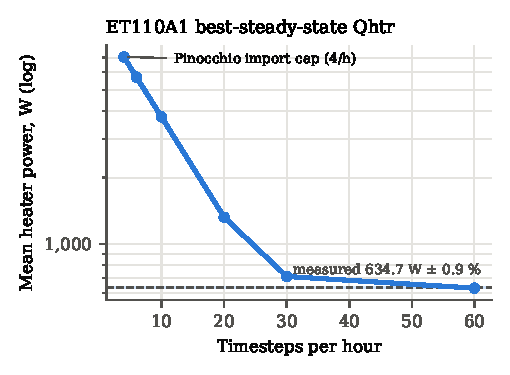
\includegraphics[width=0.52\textwidth]{figures/fig_etna_timestep.pdf}
\caption{ET110A1 heater power as a function of time step. The \emph{only} physical change Pinocchio-EP's import path
makes to the ETNA model is Timestep 60$\rightarrow$4 per hour. An object-by-object diff of the two IDFs found no
other difference besides the table-output style.}\label{fig:etna}
\end{figure}

Run directly on Pinocchio-EP's engine, the four ``1'' cases match the measured mean within the uncertainty band,
consistent with the published EnergyPlus~23.1 example results. The hourly scatter is larger than measured (standard
deviation 5--8\,W against 2--3\,W), so only 28--78\,\% of hours lie individually inside the band. Two engine-level
anomalies apply to every Pinocchio-EP user:
\begin{enumerate}[label=(\alph*)]
\item EnergyPlus~26.1 accepts the IDD keys \code{FisherPedersenCeilingDiffuserWalls}/\code{Ceiling} in
\code{SurfaceProperty:ConvectionCoefficients:MultipleSurface} but stops with ``Unhandled convection coefficient
algorithm''. The informative ET100A3/B3 inputs, which ran under version~23.1, cannot run, and the nearest runnable
variant is 8\,\% high.
\item The Denver runs report psychrometric non-convergence warnings (wet-bulb of very dry air at 82\,kPa). They
are harmless here but should be documented in block~G.
\end{enumerate}
Through Pinocchio-EP's import path the same models over-predict heater power by 293--1043\,\%
(Figure~\ref{fig:etna}). With roughly 21 air changes per hour of measured supply air and a fine time constant, the
ideal-loads zone balance needs 30 to 60 steps per hour. Capping the time step at 4 makes the result meaningless.
Addendum~b's new clause 5.1.1.9 places time-step choice with the software implementation, so silently overriding
the modeller's setting is a non-conformance. In addition, the deployed service uploads only \code{in.idf}, so
\code{Schedule:File} boundary data never reach the engine.

\section{Clause-by-clause conformance matrix}\label{sec:matrix}
{\small
\begin{longtable}{p{3.2cm}p{2.3cm}p{10.2cm}}
\toprule Requirement & Status & Evidence (measured, or from code)\\\midrule\endfirsthead
\toprule Requirement & Status & Evidence\\\midrule\endhead
Unmodified, versioned calculation engine & \OK & Official NREL EnergyPlus 26.1.0-6f2e40d102. The server writes \code{idf\_text} verbatim; no rewriting (\code{server.js:353-395}).\\
5.1.1.1 Time convention, no DST or holidays & \PART & EPW is passed unshifted. Starter RunPeriod defaults to weather-file DST \emph{Yes} and holidays \emph{Yes} (\code{starterIdf.js:39-42}); editable only in the objects editor.\\
5.1.1.4 Consistent numerical settings & \NO\ (import route) & The import path overrides the modeller's time step (cap 4/h). For ETNA this changes $Q_{htr}$ by up to 1043\,\%.\\
5.1.1.5/5.1.1.6 Equivalent and nonspecified inputs documented & \PART & A provenance system exists (value basis), but there is no record of EnergyPlus defaults that applied (convection, shadowing, CTF) and no S140outNotes generator.\\
5.1.2 / Annex A2 reporting & \NO & No \code{Std140\_*\_Output} export, no \code{S140outNotes}, no application version identifier (block A needs one; only the EnergyPlus version is recorded).\\
Annex A3 no-proxy rule & \NO\ (not yet tested) & No Pinocchio-EP submission exists. EnergyPlus's own results cannot be cited.\\
Section 6 weather drivers & \NT; \PART & EPW import only. TMY3/TMY2/TMY/WYEC2 are not accepted. Site and ground reflectance come from the EPW. Incident-solar outputs for arbitrary tilt need Output:Variables the GUI cannot add.\\
Section 7 low mass & \OK\ (indicative) & P/I 34/34; G 33/34 (needs 30). Substitute weather file.\\
Section 7 high mass & \PART & P/I 28/28; \textbf{G 21/28 (needs 25)}. GUI windows are simple glazing only.\\
Section 7 cases 450--470 (constant coefficients) & \PART & Not creatable in the GUI (\code{SurfaceProperty:ConvectionCoefficients}); possible only via import.\\
Section 7 terrain (7.2.1.9.1) & \NO\ (GUI) & Terrain hard-coded ``City''; the ``Site exposure'' field is not exported. This alone puts 600 (G) and 900 (P) out of range.\\
Section 7 free-float & \PART & The GUI refuses runs with no conditioned zone (\code{EpWorkspace.jsx:997}). The emitter produces them correctly.\\
Section 7 output (7.3) & \PART & The Results view converts ideal-load cooling with COP~3.5 and has no hourly-variable selection or peak time stamps. Raw CSV download is capped at 12\,MB per file.\\
Section 8 ground coupling & \NT; \PART & Default slab = constant monthly ground temperature. Kiva, GroundDomain and the Slab preprocessor are import-only, and a Kiva boundary is lost if the zone is edited.\\
Sections 9--11 HVAC equipment & \NT; \PART & DX coils, furnaces and FC/CV/VAV systems exist in Pinocchio Studio, but there are no performance-map fitting, TMY2/WYEC2 weather or node-level outputs in the GUI. No CE/HE/AE run was made.\\
Section 12 Class II & \NT & Not attempted (TMY weather, attic and basement models).\\
Section 13 ETNA (engine) & \OK\ (1-cases) / \NO\ (3-cases) & Direct engine: within $u$ on the means. ET100A3/B3 inputs are fatal on E+~26.1.\\
Section 13 ETNA (Pinocchio route) & \NO & Time-step cap (+293 to +1043\,\%). Schedule:File data not uploaded. OtherSideCoefficients and Output:Variables not creatable in the GUI.\\
\bottomrule
\end{longtable}}

\section{Where Pinocchio-EP does not follow the standard, and how to fix it}\label{sec:gaps}
\begin{enumerate}[label=\textbf{N\arabic*.},leftmargin=2.4em]
\item \textbf{No Standard~140 test record exists for Pinocchio-EP.} \code{src/lib/compliance/bestest.js} holds one
regression case (\code{1ZoneUncontrolled}), and Case~600/900 are commented out. The runner sends an EnergyPlus
example file straight to the engine and never touches Pinocchio-EP's emitter. \emph{Fix:} promote
\code{harness/} from this study into \code{tools/} as a CI gate that runs Sections~7 and 13 through
\code{exportIdf} on every release.
\item \textbf{Window model in the GUI is simple glazing only.} This causes the high-mass failure (900 cooling, 950,
960, 980 cooling, the 940/980 day curves) and the 695 RMSE failure. Standard~140 informative 4.5(c) notes that a
citing organisation may require testing with the inputs users actually enter. A citing organisation applying that
guidance would grade the G route, and it fails. \emph{Fix:} add a layered-glazing editor (\code{WindowMaterial:Glazing}
and \code{:Gas} from the IGDB/WINDOW data) and make it the default for code-compliance projects.
\item \textbf{Terrain is hard-coded ``City'' and the ``Site exposure'' field is dead} (\code{starterIdf.js:33};
nothing reads \code{project.terrain}). \emph{Fix:} write \code{Building\,\textgreater\,Terrain} from the field and
default it to ``Suburbs'' or ``Country'' according to site type.
\item \textbf{The import path overrides the modeller's time step} (\code{idfSync.js:168-171}). \emph{Fix:} remove the
cap, or warn and require confirmation. Never change numerical settings silently (5.1.1.4, 5.1.1.9).
\item \textbf{Objects that 140 inputs need cannot be created in the GUI:} convection coefficients,
\code{Output:Variable}, \code{ZoneVentilation}, \code{OtherEquipment}, free-form shading,
\code{SurfaceProperty:OtherSideCoefficients}, \code{Foundation:Kiva}, \code{HeatBalanceAlgorithm},
\code{ShadowCalculation}. \emph{Fix:} add ``add object'' with IDD validation to the objects editor, or dedicated
panels.
\item \textbf{Defaults that contradict the specification without telling the user:} material solar absorptance
0.7 (\code{constructionLib.js:234-262}); re-assigning a construction wipes material edits; ideal loads with
dehumidification at SHR~0.7 (Standard~140 requires no latent extraction); Solar Distribution FullExterior;
RunPeriod DST and holidays on. \emph{Fix:} a ``Standard~140 / validation'' project profile that sets the
specification values and records them.
\item \textbf{Weather handling.} EPW only. There is a silent fall-back to the Golden~CO file when an uploaded EPW
has been swept (14 days). \emph{Fix:} accept TMY3 CSV and TMY2 through EnergyPlus's converter, archive the
converted file with the run (5.1.2.2), and fail loudly instead of falling back.
\item \textbf{Outputs and reporting.} The Results view's cooling ``energy'' is ideal load $\div$ 3.5. There is no
hourly-variable picker, no peak time stamps, no Std140 workbook export and no S140outNotes. Downloaded files are
capped at 12\,MB. The application has no version identifier. \emph{Fix:} a ``Std140 report'' export that fills the
normative workbooks and the A--G notes from the run, stamped with a build version.
\item \textbf{Free-float runs refused} when no zone is conditioned (\code{EpWorkspace.jsx:996-997}).
\emph{Fix:} allow unconditioned runs with a warning.
\item \textbf{Deployed runs cannot carry side files.} \code{Schedule:File} CSVs are never uploaded, so ETNA (and any
measured-data calibration) cannot run in production. \emph{Fix:} inline the data as \code{Schedule:Compact} on
import, or upload attachments with the IDF.
\item \textbf{Engine anomaly to report upstream.} FisherPedersen ceiling-diffuser keys are accepted by the IDD
but fatal in E+~26.1. Until this is fixed, ET100A3/B3 cannot be modelled as specified on Pinocchio-EP's engine.
\item \textbf{Untested sections.} 6, 8, 9, 10, 11 and 12. The HVAC Studio (an openstudio-standards replica) contains
the needed component types, but the CE/HE/AE groups require user performance maps, part-load curves and constant
TMY2/WYEC2 conditions that no GUI path currently provides.
\end{enumerate}

\section{Summary: how much of the standard does Pinocchio-EP follow?}
\begin{itemize}
\item \textbf{Physics engine.} EnergyPlus~26.1 is used unmodified. With faithful inputs it reproduces the
Section~7 acceptance ranges completely and the ETNA ``1'' cases within measurement uncertainty.
\item \textbf{Through its own IDF writer.} Pinocchio-EP preserves the inputs faithfully. Cases built through
\code{exportIdf} and through IDF import give identical annual loads (to 0.001\,MWh) and pass both thermal-fabric groups
(62/62 range cases).
\item \textbf{Through its own GUI.} Only one of the two thermal-fabric groups passes (low mass 33/34; high mass
21/28), and out-of-the-box defaults (terrain City) push even Case~600 out of range.
\item \textbf{Coverage.} Of the five acceptance-graded test groups, two were exercised and three (cooling,
heating and air-side equipment) were not. The informative Sections~6, 8 and 12 were not run. Section~13 fails
through Pinocchio-EP's import path.
\item \textbf{Formal status.} No submission exists, the required output reports cannot be produced, and the
software has no version identifier. Pinocchio-EP does \emph{not} currently conform to Standard~140-2023. It is
close on the thermal fabric once N2--N4 are fixed.
\end{itemize}

\section{Limitations}
The Section~7 weather file is a substitute derived from the same TMY3 record, so small differences from the
normative \code{725650TY.CSV} are possible. Results near range limits (900 cooling 2.377 against a 2.35 lower
limit) should be re-run with the normative file. The ETNA engine runs reuse the informative EnergyPlus inputs, which
Addendum~b says are not to be used for new results. They establish engine behaviour and the effect of Pinocchio-EP's
import path, not a Section~13 submission. The G route models a careful user. A user who keeps every default does
worse (Table~\ref{tab:sens}). The CE, HE, AE, GC, WD and Class~II suites, and the inside-surface flux outputs of
Section~13, were not run.

\appendix
\section{Draft S140outNotes content for a future submission (Section 7)}
\begin{description}
\item[A. Software.] Pinocchio-EP (web, ERGO Energy LLP), build \emph{to be stamped}; engine EnergyPlus 26.1.0-6f2e40d102;
browser client plus Linux server.
\item[B. Alternative methods.] Inside convection TARP and outside DOE-2 (EnergyPlus defaults); CTF conduction;
PolygonClipping shading every 20 days; full interior and exterior solar distribution; third-order backward-difference
zone air balance; 4 time steps per hour.
\item[C. Equivalent methods.] Floor insulation as \code{Material:NoMass} R = 25.075/25.175 (zero capacitance);
ideal loads through \code{HVACTemplate:Zone:IdealLoadsAirSystem} with sensible-only output variables; Case~640
ramp by linear interpolation in 15-minute steps, with the 23:00 step-down within one time step.
\item[D. Nonspecified inputs.] Visible glazing properties set equal to solar values (no effect on loads).
\item[E. Omitted cases.] In-depth cases 195--470, 800 and 810 were not run in this study.
\item[F. Source changes.] None.
\item[G. Anomalies.] Psychrometric wet-bulb non-convergence warnings (two occurrences per run).
\end{description}

\section{Reproducibility}
All scripts and result data are in this folder: \code{harness/suite.mjs} (case builder, run with
\code{node suite.mjs all P,G}), \code{harness/roundtrip.mjs} (import route), \code{harness/score.py} (Annex~A3
scoring), \code{harness/run\_etna.py} and \code{harness/via\_pinocchio.mjs} (Section~13), and
\code{harness/figures.py}. Results are in \code{data/*.json}. Paths inside the scripts point at the original
scratch directory and must be adjusted.

\begin{thebibliography}{9}\small
\bibitem{s140} ANSI/ASHRAE Standard 140-2023, \emph{Method of Test for Evaluating Building Performance Simulation Software}. ASHRAE, 2023.
\bibitem{s140a} ANSI/ASHRAE/IBPSA Addendum a to Standard 140-2023 (time-series acceptance criteria), approved 29 Aug 2025.
\bibitem{s140b} ANSI/ASHRAE/IBPSA Addendum b to Standard 140-2023 (Section 13, building thermal fabric empirical validation), approved 24 Apr 2026, with accompanying files 140-2023-B (Feb 2026).
\bibitem{eplus} U.S. DOE, \emph{EnergyPlus 26.1.0 Input/Output Reference}, 2026.
\bibitem{owb} climate.onebuilding.org, \emph{USA\_CO\_Denver.Intl.AP.725650\_TMY3} (EPW of NREL TMY3 station 725650).
\end{thebibliography}
\end{document}
